\chapter{Discussion \& perspectives}
\label{ch:discussion-perspectives}
{\hypersetup{linkcolor=GREYDARK}\minitoc}

As a legacy of the nearly-neutral theory, the evolution of molecular sequences is seen as a stochastic process.
One component of this process is creating diversity through mutation, while another antagonistic component is filtering out this diversity through selection, and finally the balance between these components is arbitrated by drift.
In the long term, this stochastic process results in a history of substitution events along species trees, inducing compllex patterns of molecular divergence between species.
By analysing them, phylogenetic codon models aim at capturing the intrinsic parameters of evolution.

In this context, this thesis has been focused on phylogenetic codon models, and on modelling the interplay between mutation, selection and drift shaping protein-coding DNA sequences.
As an introduction of this conclusive chapter, I first recall the main results of this thesis in section~\ref{sec:summary-of-main-results}.

Even though the results presented in this thesis are modest, and are based on several strong and potentially questionable assumptions, these development recruited knowledge and insights from different theoretical, methodological and empirical scientific disciplines.

First, I attempt to discuss the limitations of this work.
One main in terms of the modelling of site-interdependence in section~\ref{sec:epistasis-and-entrenchment}.
Secondly, I draw the connexion between detection of adaptive evolution and the results of this work~\ref{sec:adaptative-landscape}.
As a perspective, I discuss how phylogenetic mechanistic models can be unified with population-genetics in section~\ref{sec:mechanistic-and-phenomenological-models}, and the theoretical methodology of inference that would be adapted for such endeavor in section~\ref{sec:mechanistic-and-phenomenological-models}.
Finally, before concluding, I discuss the question and issue of reproducible sciences in evolutionary biology in section~\ref{sec:reproducible-science}.


\section{Summary of main results}
\label{sec:summary-of-main-results}

Because the composition of protein coding DNA sequences does not reflect the underlying mutational process, but its filtering by selection at the level of amino-acids, a careful phenomenological modeling is necessary to uncover mutational process and nucleotide fixation biases.
Unfortunately, phenomenological \gls{codon} models developed to estimate the rate of evolution on amino-acids use the observed mutational bias at the protein level and don't take into account this effect.
As as results, \gls{codon} models in their current form are inherently misspecified to untangle mutation and selection, and they don’t estimate the mutational process reliably, even if are able to estimate quite reliably the global fixation bias acting on amino-acids.
In chapter~\ref{chap:NucleotideBias}, we developed a phylogenetic codon model where the rate of evolution is seen as a tensor (95 parameters) instead of a single parameter.
We demonstrate that this modelling approach allow also estimate reliably the mutational process, and disentangle fixation bias in different directions.

The first manuscript articulated mutation and mutation in phenomenological codon models.
However, the balance between the forces of mutation and selection is arbitrated by genetic drift, which in turn is mediated by effective population size ($\Ne$).
As a result, theoretically, variations of $\Ne$ along of a phylogeny can be estimated from the trails of substitutions along the lineages.
In chapter~\ref{chap:MutSelDrift}, we developed an mechanistic extended mutation-selection model reconstructing site-dependent fitness landscape, long-term trends in effective population size and mutation rate along the phylogeny, from an alignment of DNA coding sequences.
Together, we estimated the correlation between reconstructed life-history traits, mutation rate and effective population size, intrinsically including phylogenetic inertia.
Our framework was tested against simulated data, and empirical data in mammals, isopods, primates and drosophila.
There is persistent signal in substitution patterns that relates to past drift, and the trend in variation of effective population size can be estimated, and related to life-history traits or ecological variables.
However, the magnitude of inferred $\Ne$ across the phylogeny is narrower than expected, probably due to assumptions made on the fitness landscape.

The second manuscript leveraged the trails of substitutions along the lineages to estimate variation in $\Ne$, under the premise that lineages with large $\Ne$ are expected to undergo stronger purifying selection, thus a lower average fixation bias ($\nu$).
However, assumptions about the underlying structure of the fitness landscape has great influence on the response of the fixation bias to changes in $\Ne$.
Moreover, increase in protein expression level has also been found to empirically to result in decrease in the fixation bias the fixation bias , predicted by theoretical results recruiting the selection for protein stability.
As a result, in chapter~\ref{chap:GenoPhenoFit}, we derived a theoretical approximation for the response of the fixation bias to changes in both $\Ne$ and expression level, under an explicit genotype-phenotype-fitness map.
The development is generally valid for additive traits and log-concave fitness functions, but applied more specifically to protein undergoing selection for their conformational stability.
In this specific case, we predict a weak response of the fixation bias to changes in either $\Ne$ or expression level (which are interchangeable), and corroborated by simulations under more complex models.
Based on empirical data, we propose that fitness based on the conformational stability is not a sufficient mechanism to explain the amplitude of the fixation bias variations observed empirically.
However, other aspects of protein biophysics might be explored such as protein-protein interactions, which can lead to stronger response of the fixation bias to changes in $\Ne$.
A remaining gap between quantitative predictions of biophysical models and empirical observations about response of the fixation bias to changes in $\Ne$ and expression level.


\section{Site-interdependency and epistasis}
\label{sec:epistasis-and-entrenchment}

A blind spot of the mechanistic phylogenetic codon models developed in chapter~\ref{chap:MutSelDrift} is the assumption of site-independence.
This assumption is convenient, both computationally and statistically.
Computationally, each site is considered an independent Markov chain (see~\ref{subsec:mutation-limited-assumption} and~\ref{sec-intro:likelihood}).
Statistically, model can rely on mixture models to estimate site-specific amino-acid fitness profiles (see~\ref{subsec:empirical-calibration-HB}).
In contrast, from a modeling and inference perspective, accounting for epistasis is challenging both in terms of parametrization and computational complexity (see~\ref{subsec:structurally-constrained-site-interdependent-codon-models})
This complexity is the main reason why epistasis is generally ignored in phylogenetic models, and more particularly in codon models.

Empirically, however, evolutionary biologists have many reasons to believe that this hypothesis of site-independence is not adequate, especially in the context of protein biophysics (see~\ref{subsec:conformational-stability-and-epistatis}).
This approximation is problematic, and we can wonder what are the consequences of ignoring epistasis in the context of phylogenetic inference?
Pragmatically, how can we ultimately account for epistasis in inference?

Fundamentally, any model modeling fitness at the site level, without epistasis, implies a slow dynamic and a strong sensitivity of the mean fixation bias to changes in $\Ne$.
Intuitively, the slow dynamic of site-independent models is due to the waiting time until the next substitution, since the evolutionary process is mainly mutation limited (see~\ref{subsec:molecular-evolution-is-mutation-limited})
Moreover, the strong sensitivity of the mean fixation bias to changes in $\Ne$ originates in the fact that after a change in $\Ne$, each site of the sequences has to adapt independently, and change its position in the fitness landscape.
Taking into account epistasis, the burden of adapting to changes in $\Ne$ is shared by more sites, such that all of them don't have to switch their position the fitness landscape.
As a result, adding epistasis to the model imply a faster dynamic and a weaker response of the mean fixation bias to changes in $\Ne$.
This effect first explains the low magnitude of $\Ne$ variation estimated with site-independent mechanistic codon models in chapter~\ref{chap:MutSelDrift}.
Moreover, this also explains the low response of fixation bias to changes in $\Ne$ in chapter~\ref{chap:GenoPhenoFit}, because all sites of the sequences are involved in non-specific epistasis.
Empirically, it appears that susceptibility of $\nu$ to changes in $\Ne$ is between these two extremes, namely that of site independent fitness landscapes, and the other extreme of phenotype define for the whole sequence.
More likely, the ternary relation from sequence to phenotype to fitness imply several sites, but not all sites of the sequences.

If accounting for epistasis in mechanistic models of evolutions is challenging, paths for statistical methods that can account for epistasis are developed in section~\ref{sec:mechanistic-and-phenomenological-models}.


\section{Adaptive landscape and positive selection}
\label{sec:adaptative-landscape}

Another blind spot the mechanistic phylogenetic codon models developed in chapter~\ref{chap:MutSelDrift} is the absence of adaptive evolution (see~\ref{subsec:where-is-adaptation?}).
Indeed, the mutation-selection equilibrium is essentially a nearly-neutral regime.
As a result, at mutation-selection equilibrium, sequence is close to optimum and therefore, most mutations are deleterious or compensate for previous deleterious mutations that reached fixation.

This mutation-selection phylogenetic framework can however be leveraged as a null model, where deviation from this null model is seen has a signal of adaptation (see~\ref{subsec:adaptive-evolution}).
In this direction, a first mechanistic approach consider that adaptation consists in changes in the site-specific profile along some lineages, either informed by experimental mutational scanning~\citep{Bloom2017}, or estimated in lineages with a priori knowledge of phenotypic changes~\citep{Parto2018}
A second approach, hybrid between mechanistic and phenomenological models consider if the sequences are under pervasive positive selection, the fixation bias ($\nu$) of non-synonymous mutations would be higher than predicted by the purely nearly-neutral model.
This discrepancy between the mean fixation bias and the nearly-neutral expectation is captured by a gene-wide deviation parameter $\omega_*$, as in \citet{Rodrigue2016}.
This gene-wide deviation parameter $\omega_*$ can be refined at the site-level.
In this vein, in work led by Nicolas Rodrigue, we developed a method to detect site-specific adaptation as a deviation from a null nearly-neutral model of evolution.
This methods has been developed in the framework Bayescode (see~\ref{subsec:implementation}), and the manuscript is available in appendix page~\pageref{sec-appendix:MutSelM3starMBE}.
These methods are relatively new, and must remain to be applied more broadly to empirical data, such as be to compared with classical codon models.

However, in its current form, phylogenetic model seeking adaptation as a deviation from near-neutrality assumes a constant $\Ne$ across the tree.
This suggests that adding $\omega_*$ in the mechanistic-model developed in chapter~\ref{chap:MutSelDrift} would potentially be more effective at detecting positive selection.
Moreover, $\omega_*$ could also be allowed to vary across branches, alike $\Ne$.
This could have interesting applications, for instance, do bats, compared to other mammals, have both stronger purifying selection due to large $\Ne$ and stronger positive selection (larger $\omega_*$)?

Additionally, the rate of adaptive evolution estimated by phylogenetic codon models can be confronted to estimates of adaptation obtained with polymorphism dataset within species.
Originally pioneered by \citet{McDonald1991}, the ratio of non-synonymous over synonymous polymorphism ($\pnps$) supposedly contains solely non-adaptive polymorphism, under the assumption that adaptive mutations are rare.
On the other hand, the ratio of non-synonymous over \glspl{synonymous} ($\dnds$), estimated from divergence data, is supposedly composed of a mixture of both advantageous \glspl{substitution} and non-adaptive (\gls{nearly-neutral}) \glspl{substitution}.
Thus the difference $\dnds - \pnps$ is also the rate of adaptive evolution.
To note, the rate of non-adaptive evolution obtained with polymorphism data, $\pnps$, supposedly matches the compound parameters $\omega_0$ obtained uniquely from divergence data.
However, estimation of adaptive rate can be biased by moderately deleterious mutations and by the change in population size through time~\citep{eyre-walker_changing_2002}.
To overcome this biases, the method of \citet{eyre-walker_estimating_2009, Galtier2016} relies on the synonymous and non-synonymous site-frequency spectra (\acrshort{SFS}) to estimate the distribution of fitness effects of mutations (\acrshort{DFE}), modeled as a continuous distribution.
Subsequent development of these methods are reviewed in~\citep{Moutinho2019a}, intrinsically measuring the rate of non-adaptive evolution present in polymorphism data.

From the availability of divergence and polymorphism data, it is now possible to ask whether the rate of non-adaptive evolution measured by phylogenetic mutation-selection models matches the rate estimated from \acrshort{SFS}.
Are phylogenetic \gls{codon} models and population-genetics models independently estimating the same rate of adaption?
And if not the reason for such discrepancy should be understood.

\begin{figure}[H]
    \centering
    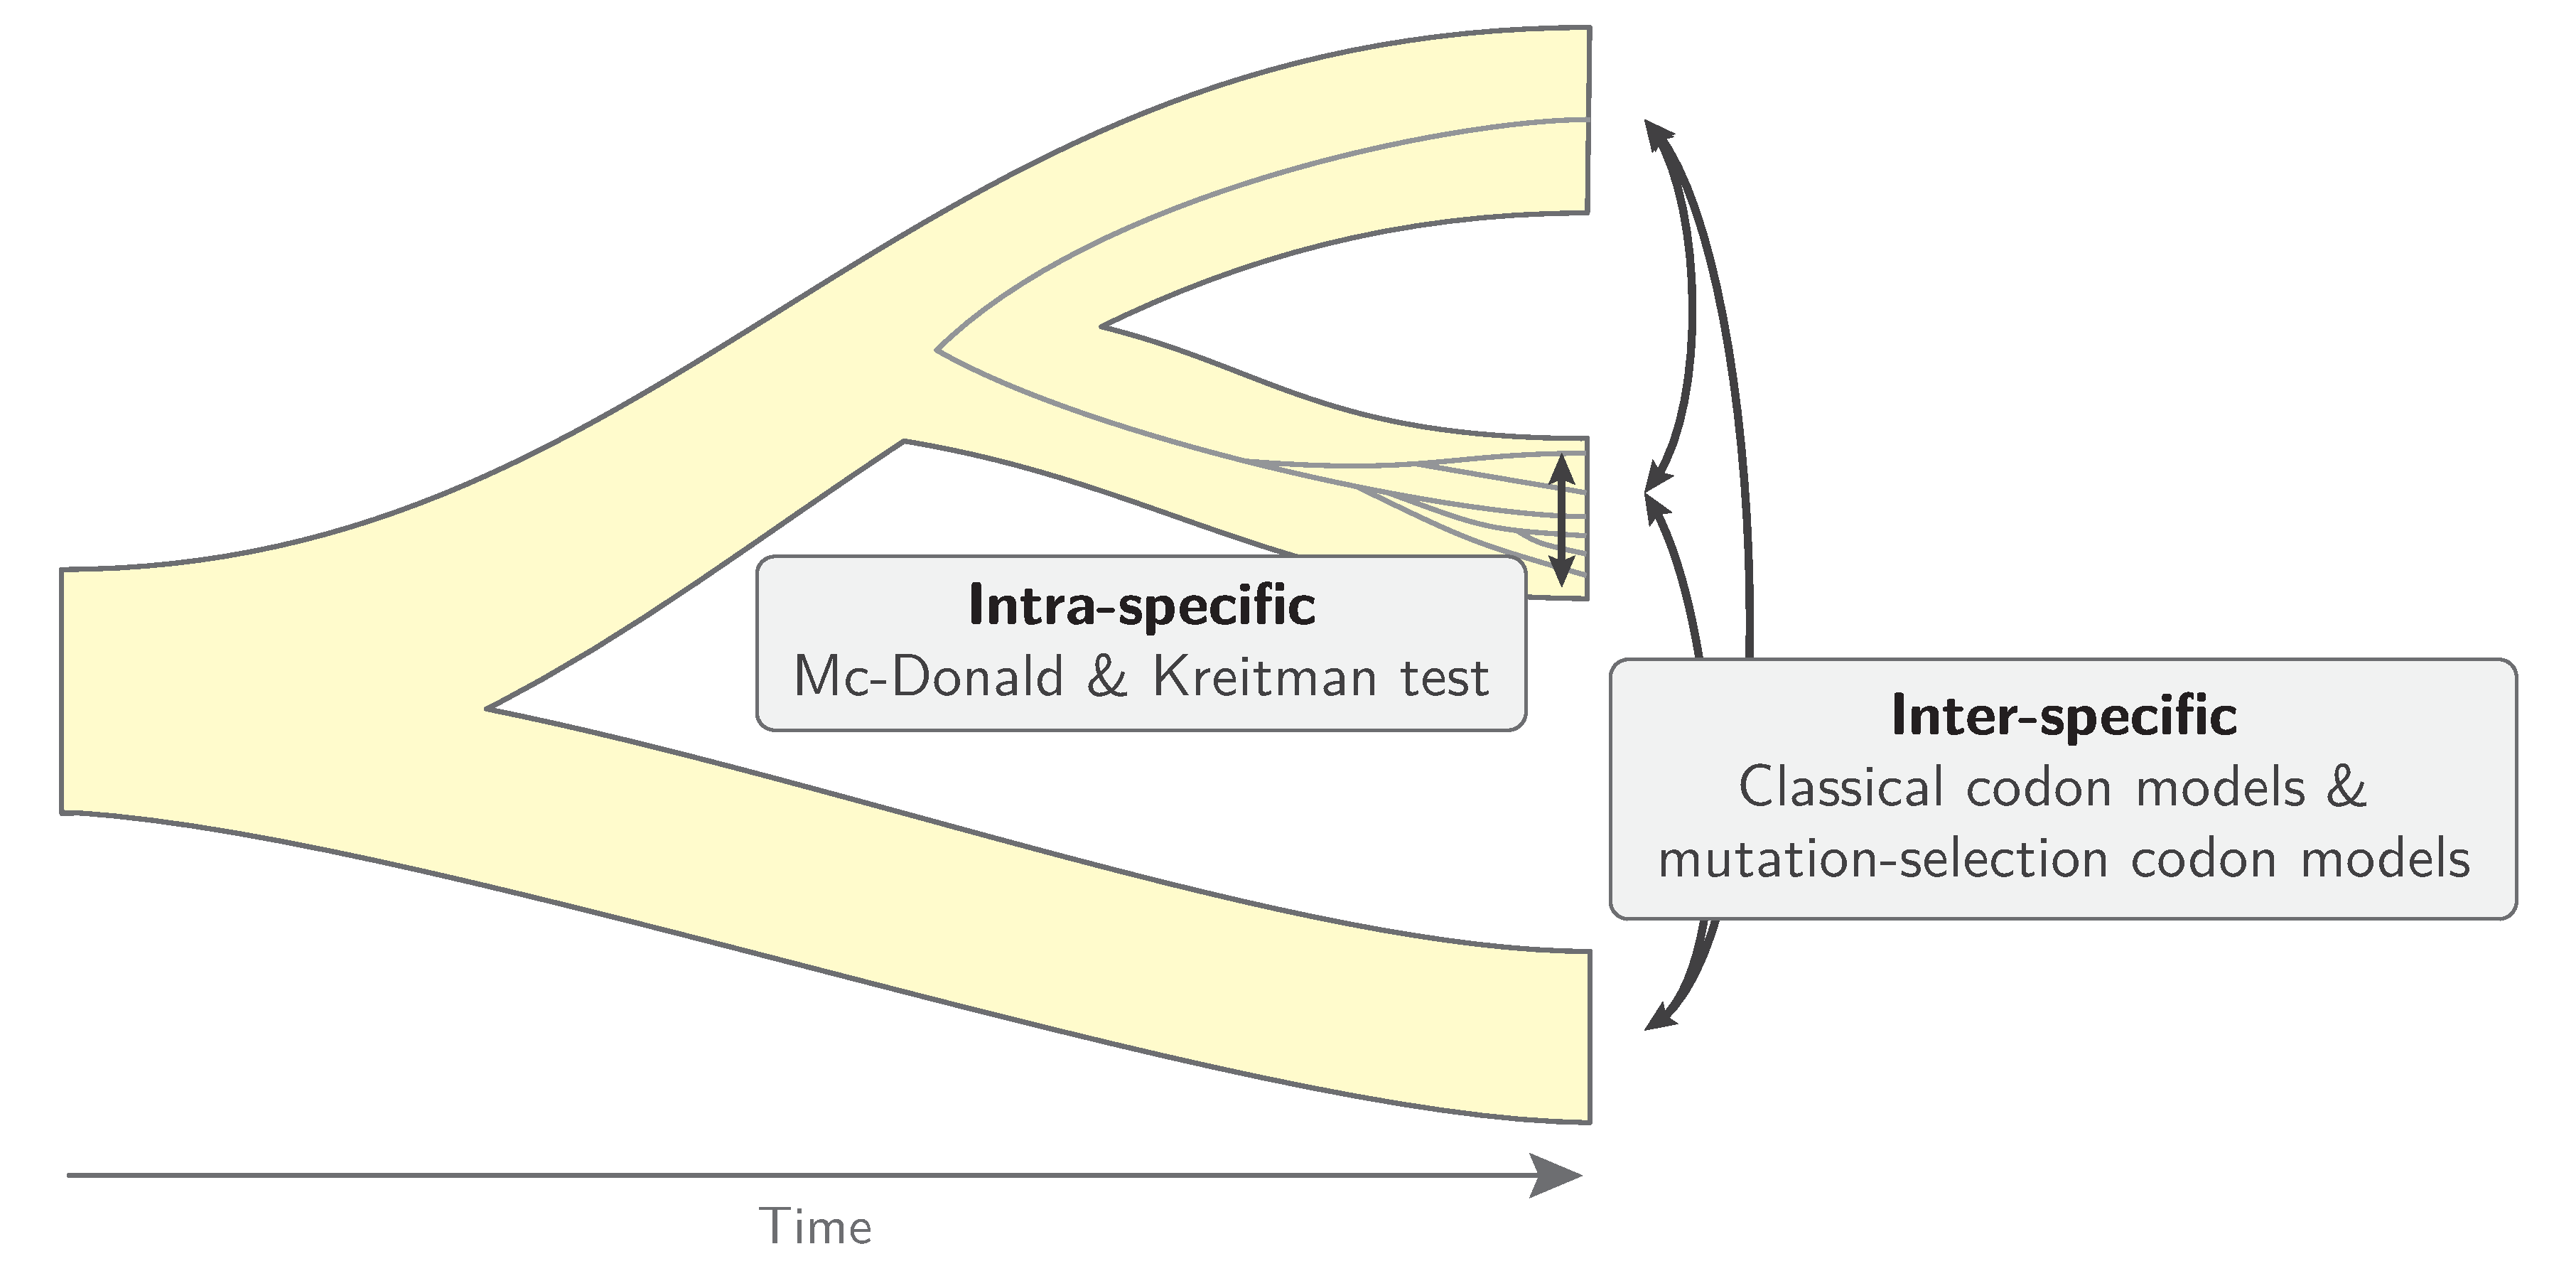
\includegraphics[width=\textwidth] {figures/inter-intra}
    \caption{Detecting adaptive evolution in coding sequences from inter- and intra-specific data}
    \label{fig:detecting-adaptation-inter-intra}
\end{figure}


\section{Unifying phylogenetic and population-genetics model}
\label{sec:unifying-phylogenetic-and-population-genetics-model}

Along this manuscript, phylogenetic codon model has so far discarded diversity within species, and polymorphism has not been leveraged.
As a result, all divergence observed in the alignment are assumed to be substitutions.
However some substitutions might be polymorphisms in the population but appear fixed in the sampled individuals.
Moreover, substitution are not instantaneous and ancestral shared polymorphisms can result in incomplete lineage sorting~\citep{Charlesworth2010}.
As a result, mistaking substitutions and polymorphisms is problematic since both are not sensitive to mutation, selection and drift in the same extent~\citep{Mugal2014}.
For example, the number of polymorphisms (diversity) increases with $\Ne$, while rate of neutral substitutions is insensitive to $\Ne$.
Also, mildly deleterious can be present in polymorphism while being filtered out by selection and not present in substitutions.
In contrast, mutational bias is entangled with selection in substitution (see chapter~\ref{chap:NucleotideBias}), while being more easily detectable in polymorphism.
As a result, polymorphism and divergence can be leveraged altogether to help disentangle mutation, selection and drift.
As such we can wonder whether phylogenetic and population-genetics model can be unified?
% Charlesworth, D. (2010) Don’t forget the ancestral polymorphisms. Heredity, doi:10.1038/hdy.2010.14

Such integration between phylogenetic and population-genetics as been proposed \citep{Thorne2012} and attempted in severals studies.
For example, \citet{Wilson2011} modeled codon evolution in a joint framework with $3$ species, allowing to analyze variation in selection pressures spatially along the genome and temporally between lineages.
This methodology proved to be computational intensive and scaled difficulty with the number of extant species.
Alternatively, modeling substitutions as mutational events followed by a gradual fixation allow to estimate nucleotide mutation rates and fixation biases from genetic variation within and between species, inherently accounting for shared ancestral polymorphisms and incomplete lineage sorting~\citep{DeMaio2013, Schrempf2016, Bergman2018, Schrempf2019}.
Hence, this methodology can be leveraged to disentangle gBGC and mutational bias~\citep{Borges2019, Borges2020}, although this methodology scale difficulty with the number of states of the models, and would be difficult to translate from a nucleotide matrix (4 states) to a codon matrix (61 states).

Because mechanistic \gls{codon} models are based on population-genetics first principles, they can theoretically be extended to account for within species diversity.
The strategy can be to augment molecular divergence data between species with information about molecular polymorphism within species.
Such attempt has been tried during the first year of the PhD, where the formalism, based on Poisson Random fields can be found in appendices page~\pageref{sec-appendix:PRF}.
This extension was rather straightforward to implement into BayesCode, extending site-specific mechanistic codon models.
A first implementation provided sensible estimation of diversity ($\theta = 4 \Ne u$) based on generated simulation under Wright-Fisher model of evolution.
Alas, it was found to be computationally intensive, even though optimizing the computation with sufficient statistics.
Moreover, the assumption of constant $\Ne$ along the phylogeny assumed by mutation-selection codon models was arguably the strongest assumption to relax in such context.
In other words, what sense would it make to integrate diversity in extant species that generally have quite different levels of diversity if $\Ne$ is considered constant along the phylogeny.
It was historically the reason to extend phylogenetic site-specific mutation-selection \gls{codon} models by incorporating branch-specific $\Ne$, presented in chapter~\ref{chap:MutSelDrift}.
After extending mutation-selection with branch specific drift, we actually realized that the susceptibility of \gls{substitution} rate to changes in $\Ne$ is too strong because of site-independence assumption (chapter~\ref{chap:GenoPhenoFit}), effectively amortizing the range of $\Ne$ which could be inferred.
Moreover, with branch-specific $\Ne$ and extant polymorphism, the computing time to reach convergence of the MCMC became prohibitive.

Finally, even tough site- and branch-specific mutation-selection phylogenetic \gls{codon} models can be extended by incorporating signal of polymorphism, which actually has been implemented in Bayescode, I believe it is not yet the path forward to build an unified phylogenetic and population-genetics model.
Before being unified, I believe phylogenetic codon models and population-genetics method should be confronted, and the discrepancy should be understood, such as presented in the previous section.
As a second step, subsequently to this confrontation, phylogenetic models could in principle accommodate extant polymorphism, but they will require another approach of inference more computationally reasonable.


\section{Mechanistic and phenomenological models}
\label{sec:mechanistic-and-phenomenological-models}

% Categories of models
Models of inference are classified broadly into phenomenological and mechanistic~\citep{Rodrigue2010a}.
Mechanistic models dissect the causation chains and construct a model from first principles, they relate structural, population-genetics and ecological parameters to the \gls{likelihood} of the data (see chapter~\ref{chap:MutSelDrift}).
As such, mechanistic inference models are suitable to construct an integrative framework, for example relating the signal available in molecular sequences to structural parameters, expression level across genes and \gls{effective-population-size} across lineages.
Once such models is fitted to the data, the estimated parameters can be confronted to their independent empirical estimate, which allow to robustly test the model since orthogonal estimation of biological and ecological parameters should be congruent~\citep{Dasmeh2014}.
Additionally, once model robustness has been assessed, this inference framework could allow to estimate unknown variable, for example ancestral \gls{effective-population-size}, with enough signal and calibration of the other parameters.
However they are computationally intensive and some simplifying assumption (such as no epistasis) can have detrimental effects (see chapter ~\ref{chap:MutSelDrift}).

On the other hand phenomenological models are based on aggregate parameters of evolution, and aims to determine the statistical significance of these parameters.
As experienced in chapter~\ref{chap:NucleotideBias}, mean-field phenomenological models are useful tools to disentangle mutation and selection, such that gene specific mean-field parameters can capture and aggregate site-specific parameters.
In between phenomenological and mechanistic, models can be hybrid, mechanistic in essence, but subsequently phenomenological by deriving aggregate parameters of evolution from underlying microscopic parameters (see chapter ~\ref{chap:GenoPhenoFit}).

Observations and experiences done throughout this thesis led to crystallize the conception that models of inference should be mechanistic in essence, in the sens that they should be parameterized by variables that can be obtained from other independent experiments.
In order to be more realistic, they should be complexified by introducing various sources of variability, for example incorporating site-interdependence or polymorphism within species.
However, they should not simply add more parameters and more computational intensive algorithm.
First because of the limit of computing power available, but apart from the physical limit, they should be as parsimonious as possible in the use of computing resources since any computation bears ecological consequences on environmental degradation and $C0_2$ emissions.
Moreover, increased complexity of the model bears another consequences, such that the liability of the code and software decreases, hence the reproducibility of such models.
Altogether, hybrid models based on mechanistic first principles but deriving analytically aggregate parameters are avoiding the pitfalls of both, being based on independently identifiable parameters and at the same time being computationally parsimonious.
Such endeavor however requires an intensive labor to derive the relationship between parameters of interest (such as $\Delta \Delta G, \Ne, $ expression level, \ldots) and aggregate parameters of evolution that are extractable from the data ($\nu$).


\section{Reproducible science}
\label{sec:reproducible-science}

This thesis is based on a combination analytical models, computational simulations and inference models, which I argue are complementary, but more importantly they are necessary to each others.
Theoretical modeling allow to understand the principles, simulations allow to verify the soundness.
Inference allow to extract and test the theoretical results using empirical data, also verified and test against simulations.
Simulations have a dual role, testing the robustness of both inference procedures and theoretical results, outside of their comfort zone and assumptions.
However, this assume we are confident enough to write reproducible computations, as such the next section is dedicated to my personal experience in reproducing results.

First, I stand firmly on the ground that data, codes and scripts should be rendered open-access of any published and peer reviewed paper.
Practically, the availability of the data and source code should simply be enforced upon submission to journal, which is currently not the case for all journals, even in bio-informatics and genomics fields.
It is true that such enforcement bears the consequence to weight more burden on scientists upon publishing.
However, it avoids the bloating of technical debt, or research debt where we build on the ground of a dangerous and possibly shaky basement.
It encourages peer collaboration, both helping the team or person whom made the code available, and the community as a whole.
A straightforward way is to provide a \textit{git} versioned repository, with the advantage that collaboration is facilitated trough web hosted repository such as GitLab (hosted by institutions) or GitHub (hosted by Microsoft).

Nonetheless, code availability is a necessary condition, but not the sole requirement of reproducible research.
Specific instructions to reproduce the results should also be made available, where many tools are available to this aim~\citep{Wilson2014,Darriba2018}.
The first step necessary to reproduce a code is to have the required environment, meaning the necessary libraries and dependencies for the code and scripts.
For script and code written in Python, the package manager anaconda (or conda) provides a readily available environment to configure the necessary libraries with their versions.
More complex environment requiring code compilation or system-level packages can leverage containerization technology such as Docker or Singularity for example, but any other containers implementing system-level virtualization is very helpful to provide the necessary libraries.
Once the environment is specified, the documentation can be made available as a README with the necessary instructions.
More generally, notebooks such as \textit{Jupyter Notebook}, \textit{RMarkdown} or \textit{org-mode} to name a few also provide an environment knitting together code and instructions, allowing to follow step-by-step experiments, analysis and results, in a similar fashion as laboratory notebook required in wet labs.
It is important to note that notebooks can run code from a variety of languages (C++, Haskell, Java, Julia, Python, Wolfram Language, Matlab, Ruby, \ldots).
These tools are emerging in the community, as well as Workflow management system (Nexflow, Snakemake, \ldots) allowing to create reproducible and scalable data analyses running on computing clusters.

Using this range of tools helps other scientists which might want to understand, test or build upon published works.
Moreover, they are also very helpful for the person or team implementing them since a more rigorous and reproducible environment allows to more easily track down bugs and test programs under different conditions or dataset\footnote{Notebooks are very useful to present work and data analysis, but should not be used during development since they often offers poor integration with debugger and code inspection tools, enforce awkward software design patterns, and often result in bloated versioned repository.}.
During the development period, continuous integration pipelines are valuable to increase the reliability of code generation, which should be used whether working alone or inside team, but is of course more critical for collaborative code where one cannot control all the code written.
Collaborative coding practices such as peer-coding sessions is really useful to implement critical code at the core of the program under development.
I argue that the efficiency peer-coding sessions is provided by dividing the tasks into a group focused in the detailed implementation while the others a free to focus on edge cases and the overall implication of different implementations.
Moreover, peer-coding sessions provides a convenient and structured place for learning good practices, for expanding its technical knowledge while pruning bad habits.
An other remarkable practice is to write two independent version of the program, using if possible different algorithm and languages but with the same functionality, but most importantly by a different person.
Then testing the program against each others on the same conditions and dataset should result in the same outcome\footnote{An extreme version is adversarial coding (or chaos engineering), where the goal is to find conditions on which the adversary program fails.}.
Such model of reproducible computing experiment and analysis is laborious and demanding, but I argue this is the definition of reproducibility we collectively should aim for, namely where one can independently reproduce the same experiment, and if reproducibility fails one can run the code with different conditions to pinpoint the failing code (which might actually be in both versions).
Personally, having practiced this method I strongly believe it pervasively reduces our research debt that we might inadvertently burden other with whenever not realizing the program is bugged, and ultimately save us time on debugging and research conduction.
Finally, explaining to others our choices of algorithms, implementation and data structure requires us to express intelligibly our mental ideas and therefore better understand them, while gaining from others insight and algorithmic expertise.


\section{Concluding remarks}
\label{sec:concluding-remarks}

To conclude, this work is modest attempt to construct integrated models of protein coding \acrshort{DNA} sequences evolution.
It succeeded in consolidating the idea that the patterns of \glspl{substitution} inform us on long term fluctuation of drift along branches, and selection along sites.
It did not succeeded in modeling the fitness landscape, apparently either too site-specific, or integrated over too many sites.
It is an indication that fitness landscape of protein coding sequences is between this two extremes.
It is building block to bridge phylogeny and population-genetics, constructing an integrated framework is theoretically possible but with limited scope.
However, confronting the estimation of phylogenetic \gls{codon} and population-genetics model, through for example the rate of adaptive \gls{substitution}, is a path forward in an integrated view of .
Finally, I believe this thesis is not providing any ground breaking, nor disruptive results, but instead is consolidating theoretical models on which molecular evolution is based, and points out the pitfall to avoid.
Science, alike a mutation-selection process not is optimized but as to trade off exploration of new ideas and exploitation of old ones.
Attempts to build bridges and connection between fields, alike \gls{recombination}, can bring the best of both worlds but many attempts are required.